



\chapter{Introduction to experimental designs}

In this chapter I briefly describe the major methods to extract from data treatment effects. This is not an exhaustive treatment on the matter, but is instead designed to be an introduction to the various techniques and how they can be applied in a regression framework. For example, the discussion on propensity scores does not discuss, in detail, variance estimation or measuring bias in covariates. These are both important topics and should be explored before attempting these methods.

\section{The potential outcomes framework}

What is generally known as the Rubin causal model forms the basis of evidence for concluding that some intervention is effective in influencing the outcome of some variable, $y$.  In this section, I summarize the important ideas on this topic.

We start with the simple idea that if some unit $i$ was subjected to some randomized experiment that we could plausibly observe two outcomes, one for control ($w=0$) and one for treatment ($w=1$). The first is $y_i^{\left(0\right)}$, the outcome if unit $i$ received the control condition and $w=0$. The second is $y_i^{\left(1\right)}$, the outcome if unit $i$ received the treatment condition and $w=1$.

From this, we then conclude that for the unit $i$ the {\it treatment effect} of the experiment can be noted as
\begin{equation}
\tau_i=y_i^{\left(1\right)}-y_i^{\left(0\right)}
\end{equation}

This idea forms the basis of the Rubin causal model: each unit has in fact two data points. We then generate an assignment process, $w$, that takes on two values
\begin{equation}
w_i = \left\{ \begin{array}{ll}
     1 & \mbox{if $i$ receives treatment};\\
     0 & \mbox{if $i$ receives control}.\end{array} \right.
\end{equation}
The observed value of $y$, $y^{obs}$, is then a function of the assignment variable,

\begin{equation}
y_i^{\left(obs\right)} \equiv y_i^{\left(w_i\right)} = \left\{ \begin{array}{ll}
     y_i^{\left(1\right)} & \mbox{if $w_i=1$};\\
     y_i^{\left(0\right)} & \mbox{if $w_i=0$}.\end{array} \right.
\end{equation}

This is a missing data problem. The process to find an unbiased estimate of the typical effect of treatment, or average treatment effect (ATE), depends on the assignment process, or {\it design}.

\subsection{Average treatment effects (ATEs)}

There are many processes to estimate a treatment effect. We must be specific on exactly what kind of treatment effect we wish to estimate. First, we may be interested in the population-average treatment effect (PATE), which is the expected difference across all units, regardless of actual assignment
\begin{equation}
\tau^p = E\left[y^{\left(1\right)}-y^{\left(0\right)}\right]
\end{equation}
This is a slightly different quantity than the average treatment effect specifically on the treated (PATT)
\begin{equation}
\tau_{\left(1\right)}^p = E\left[y^{\left(1\right)}-y^{\left(0\right)}\right\vert w = 1 ]
\end{equation}
For example, we may care specifically on how an intervention impacts those targeted for treatment. Of course, we often deal with samples of individuals, so we may actually be interested in sample-average treatment effect (SATE)
\begin{equation}
\tau^S = \frac{\sum_i^N\left(y_i^{\left(1\right)}-y_i^{\left(0\right)}\right)}{N}
\end{equation}
and likewise the sample-average treatment effect for the treated (SATT)
\begin{equation}
\tau_{\left(1\right)}^S = \frac{\sum_i^Nw_i\left(y_i^{\left(1\right)}-y_i^{\left(0\right)}\right)}{\sum_i^Nw_i}
\end{equation}

In many cases, these estimates all equal each other, and in most cases we are interested in ATE writ large.

\begin{table}[htbp]\centering
\caption{Potential and observed results from hypothetical experiment \label{tab:randomassignment}
\textbf{} }\begin{tabular} {@{} c c c c @{}} \\
$y_i^{\left(0\right)}$ & $y_i^{\left(1\right)}$ & $w$ & $y_i^{obs}$ \\
\hline
17&15&1&15 \\
14&15&1&15 \\
10&12&0&10 \\
9&19&0&9 \\
15&19&0&15 \\
12&23&0&12 \\
14&18&0&14 \\
6&20&0&6 \\
15&20&1&20 \\
13&15&0&13 \\
19&27&0&19 \\
11&22&1&22 \\
10&16&0&10 \\
13&15&1&15 \\
10&21&0&10 \\
18&19&0&18 \\
21&22&0&21 \\
13&17&0&13 \\
15&21&0&15 \\
11&16&1&16 \\
13&21&1&21 \\
11&19&0&11 \\
15&19&0&15 \\
22&20&0&22 \\
18&18&1&18 \\
16&25&0&16 \\
17&23&1&23 \\
16&23&1&23 \\
9&26&1&26 \\
16&20&0&16 \\
\hline
\multicolumn{4}{@{}l}{\footnotesize{\emph{} }}
\end{tabular}
\end{table}

\section{Randomized designs}

Of course, it is not possible to observe both realities $\left(y_i^{\left(0\right)}\mbox{ and }y_i^{\left(1\right)}\right)$ for each individual: a unit either gets the treatment and we observe $y_i^{\left(1\right)}$ only, or they do not and we only observe $y_i^{\left(0\right)}$. Thus, we are observing only one outcome of a set of possibilities. These possibilities increase exponentially when we consider the possibly that one unit could impact the behavior of another. {\it That is, someone recommends to not swallow the pill.} However, if we make the of stable unit-treatment value assumption (SUTVA), each unit only has two potential outcomes, $y_i^{\left(0\right)}$ and $y_i^{\left(1\right)}$.

Our observation is then governed by $w$, the assignment variable. If $w=0$, the unit is a member of the control condition and we observe only $y_i^{\left(0\right)}$. If $w=1$, the unit is a member of the treatment condition and we observe only $y_i^{\left(1\right)}$. For example, consider Table~\ref{tab:randomassignment}. This is a table of 30 units, each with potential outcomes, $y_i^{\left(0\right)}$ and $y_i^{\left(1\right)}$, which are the first and second columns respectively. The third column is the assignment variable, $w$, and the fourth column is the observed value for $y$. As you can see, which $y$ we observe depends on $w$.

If the value of $w$ is randomly assigned, that is, it is not related to any other units value of $w$ or any other variable, $x$, then we can make a reasonable estimate of $tau$, the typical effect of the treatment. For example, consider the data in Table~\ref{tab:randomassignment}. If I calculated $tau_i$ for each unit, the average would be 5.57. I can estimate this value, however, with a $t$ test or a regression model such as
\[
y_i^{obs} = \beta_0 + \beta_1w_i+e_i
\]
where $\hat{\tau}=\beta_1=5.51$, a reasonable, unbiased, estimate.

\subsection{Controls}

In general, experimental analysis welcomes the addition of control variables, $x$, if they are observed before treatment assignment and thus not affected by the treatment process. The reason for this is simple: adding predictors reduced model uncertainty and, again, if uncorrelated with treatment, reduces the variance of the effects. The key is that with random assignment the correlation between $w$ and other predictors is 0, and thus there is no variance inflation factor as in equation~\eqref{eq:olsb1varwvif}.

\subsection{Instrumental variable estimates}

However, in doing social research we must deal with human beings. Some units may not comply with assignment. For example, consider Table~\ref{tab:ivassignment}. In this table, a random assignment to treatment, $w$, was made, but unfortunately about 15 percent of the sample did not comply. The value we observe is now determined by $r$, whether they received treatment. If we fit the model above, the estimate of $\hat{\tau}=\beta_1=2.70$, which is far to low for what we know to be true.

One method of retrieving this is instrumental variables regression (see Chapter~\ref{sec:iv} for more detail). With this method, we want an estimate of
\begin{equation}
IVE=\frac{y^1-y^0}{p_2-p_1}
\end{equation}
where $p_1$ is the proportion of units assigned control but received treatment and $p_2$ is the proportion of units assigned treatment and who receive treatment.

This quantity can be estimated in a regression framework using instrumental variables regression, also know as two state least squares (2SLS). As the name implies, this procedure involves two steps. The first step is to estimate the following linear probability model, predicting receipt of treatment as a function of assignment
\begin{equation}
r_i=\gamma_0+\gamma_1w_i+v_i
\end{equation}
then, for each unit, we predict $\hat{r}_i$ based on the model. We then fit a second model
\begin{equation}
y_i=\beta_0+\beta_1\hat{r}_i+e_i
\end{equation}
where the estimate of $\beta_1$ approximates that of $\tau$. In the case of the data in Table~\ref{tab:ivassignment}, the instrumental variable estimate $\beta_1 = 5.22$, which is a lot closer.

\begin{table}[htbp]\centering
\caption{Potential and observed results from hypothetical experiment with non-compliance \label{tab:ivassignment}
\textbf{} }\begin{tabular} {@{} c c c c c @{}} \\
$y_i^{\left(0\right)}$ & $y_i^{\left(1\right)}$ & $w$ & $r$ & $y_i^{obs}$ \\
\hline
17&15&1&0&17 \\
14&15&1&1&15 \\
10&12&0&0&10 \\
9&19&0&0&9 \\
15&19&0&0&15 \\
12&23&0&1&23 \\
14&18&0&0&14 \\
6&20&0&0&6 \\
15&20&1&1&20 \\
13&15&0&0&13 \\
19&27&0&0&19 \\
11&22&1&1&22 \\
10&16&0&0&10 \\
13&15&1&0&13 \\
10&21&0&0&10 \\
18&19&0&1&19 \\
21&22&0&0&21 \\
13&17&0&1&17 \\
15&21&0&0&15 \\
11&16&1&1&16 \\
13&21&1&1&21 \\
11&19&0&1&19 \\
15&19&0&0&15 \\
22&20&0&0&22 \\
18&18&1&1&18 \\
16&25&0&0&16 \\
17&23&1&1&23 \\
16&23&1&1&23 \\
9&26&1&0&9 \\
16&20&0&0&16 \\
\hline
\multicolumn{5}{@{}l}{\footnotesize{\emph{} }}
\end{tabular}
\end{table}

\subsection{Unconfoundedness}
\label{sec:unconf}

A major assumption of the methods to estimate an ATE is that the effect of treatment, or $y^{\left(1\right)} - y^{\left(0\right)}$, is orthogonal to $w$, given covariates, $x$. Another way of saying this is that we assume ignorable treatment assignment. We can express this assumption in symbols with
\begin{equation}
\left(y^{\left(1\right)} , y^{\left(0\right)}\right) \perp w\vert x
\end{equation}
Why this assumption is so important relates to the general assumptions of regression. Suppose we only had a single control, $x$, and that it had a linear relationship with $y$. Then, without any treatment to speak of, we could have a valid model
\begin{equation}
y_i^{\left(0\right)}=\beta_0+\beta_1x_i+e_i
\end{equation}
In an experimental setting, when we observe a mix of $y^{\left(1\right)}$ and $y^{\left(0\right)}$ as $y^{\left(obs\right)}$, if $x$ is related to assignment, then it is related to some of the residuals in the model. However, so long as $e_i \perp x_i$ (that is to say the errors are uncorrelated with covariates), the following model is valid
\begin{equation}
y_i^{\left(obs\right)}=\beta_0+\beta_1w_i+\beta_2x_i+e_i
\end{equation}
where $\beta_1$ is an estimate of $\tau$, or the treatment effect.


\section{Regression discontinuity}

There are times in which random assignment is not possible or ethical. Another plausible option in these cases is to assign the treatment condition based on


\begin{table}[htbp]\centering
\caption{Example data for Regression discontinuity\label{tab:rddata}
\textbf{} }\begin{tabular} {@{} l c c c c c c c c @{}} \\
$y_i^{\left(0\right)}$ & $y_i^{\left(1\right)}$ & $a$ & $w$ & $y_i^{obs}$ & $y_i^{obs}$ (Fuzzy 1) & $y_i^{obs}$ (Fuzzy 2) \\
\hline
6.90&17.40&0.60&1&17.40&6.90&6.90 \\
3.30&12.60&-0.60&0&3.30&3.30&3.30 \\
5.10&14.40&0.30&1&14.40&14.40&14.40 \\
9.30&18.60&1.50&1&18.60&18.60&18.60 \\
8.40&17.70&1.50&1&17.70&17.70&17.70 \\
8.70&18.90&1.80&1&18.90&18.90&18.90 \\
4.50&15.00&0.30&1&15.00&15.00&15.00 \\
2.10&12.00&-1.20&0&2.10&2.10&2.10 \\
3.00&13.20&-0.90&0&3.00&3.00&3.00 \\
5.70&16.50&0.60&1&16.50&16.50&16.50 \\
5.10&15.30&0.90&1&15.30&15.30&15.30 \\
0.60&11.10&-2.40&0&0.60&0.60&0.60 \\
3.60&14.40&-0.60&0&3.60&3.60&14.40 \\
5.70&15.30&0.60&1&15.30&15.30&15.30 \\
4.50&14.10&-0.60&0&4.50&4.50&4.50 \\
1.80&11.10&-1.50&0&1.80&1.80&11.10 \\
6.30&16.50&1.20&1&16.50&16.50&16.50 \\
2.70&12.90&-0.60&0&2.70&2.70&2.70 \\
5.70&15.60&0.00&0&5.70&5.70&5.70 \\
6.30&15.90&1.20&1&15.90&15.90&15.90 \\
7.80&17.40&0.60&1&17.40&17.40&17.40 \\
2.40&12.00&-0.60&0&2.40&2.40&2.40 \\
3.90&13.50&-0.30&0&3.90&3.90&3.90 \\
5.40&15.00&1.50&1&15.00&15.00&15.00 \\
5.10&16.50&0.00&0&5.10&5.10&5.10 \\
1.20&11.70&-2.40&0&1.20&1.20&1.20 \\
5.10&15.00&0.30&1&15.00&15.00&15.00 \\
3.60&13.80&-0.60&0&3.60&3.60&13.80 \\
6.90&17.10&1.20&1&17.10&6.90&6.90 \\
3.60&13.80&-0.30&0&3.60&3.60&3.60 \\

\hline
\end{tabular}
\end{table}


\begin{figure}
   \centering
   \includegraphics[angle=0,
           width=.75\textwidth]{rd_scatter.eps}
   \caption{Scatter plot of $y_i^{obs}$ by $a$ for data in Table~\ref{tab:rddata}}
  \label{fig:rd_scatter}
\end{figure}

\begin{figure}
   \centering
   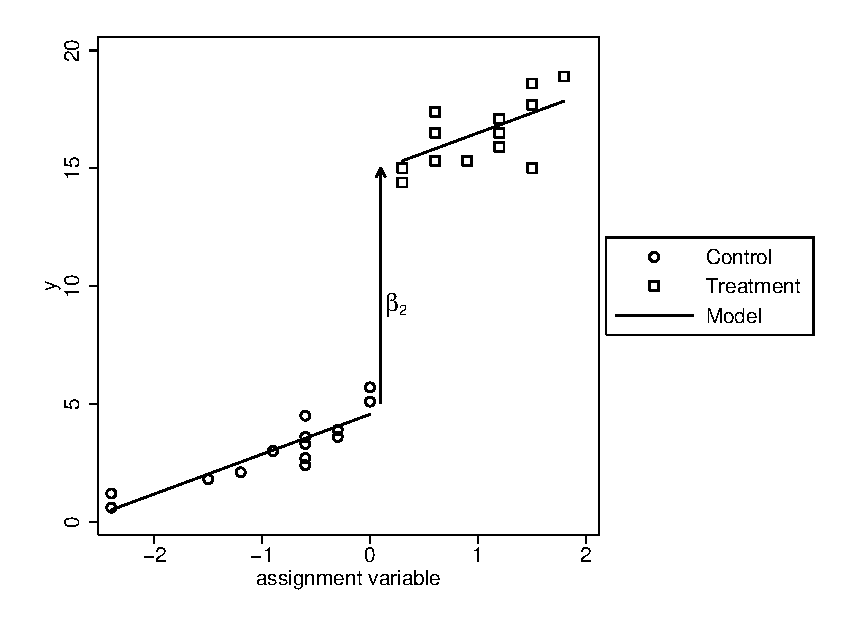
\includegraphics[angle=0,
           width=.75\textwidth]{rd_fit.eps}
   \caption{Scatter plot of $y_i^{obs}$ by $a$ with model detail for data in Table~\ref{tab:rddata}}
  \label{fig:rd_fit}
\end{figure}


\begin{figure}
   \centering
   \includegraphics[angle=0,
           width=.75\textwidth]{rd_t1.eps}
   \caption{Scatter plot of $y_i^{obs}$ (Fuzzy 1) by $a$ for data in Table~\ref{tab:rddata}}
  \label{fig:rd_t1}
\end{figure}

\begin{figure}
   \centering
   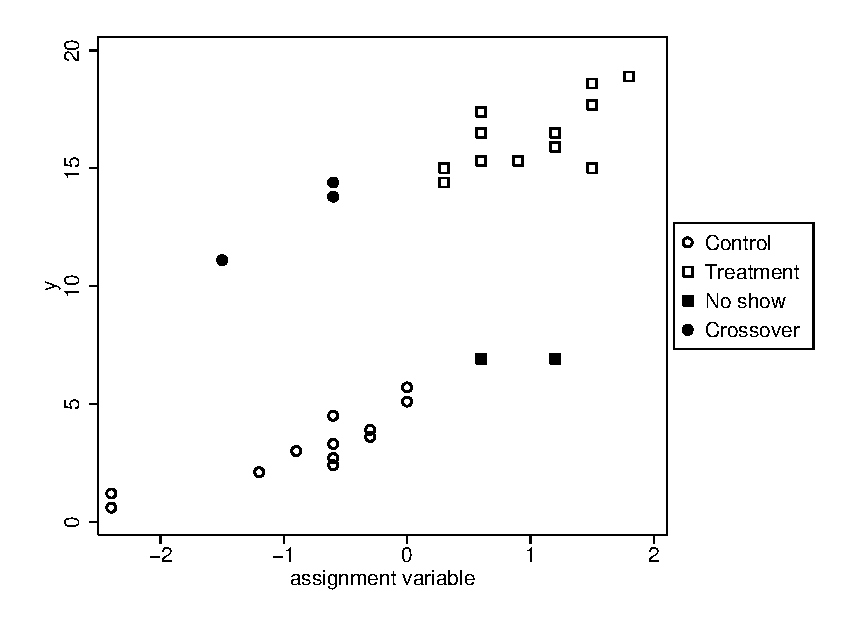
\includegraphics[angle=0,
           width=.75\textwidth]{rd_t2.eps}
   \caption{Scatter plot of $y_i^{obs}$ (Fuzzy 2) by $a$ for data in Table~\ref{tab:rddta}}
  \label{fig:rd_t2}
\end{figure}


\section{Interrupted times series}

\subsection{Splines}

\section{Difference in difference}

\section{Propensity scores}

In \ref{sec:unconf} I discuss the assumption of unconfoundedness, or that the assignment of $w$ was unrelated to covariates. In many cases where there is no random assignment, this assumption is not true. This is a situation in which $w$ is plausibly a function of other covariates. For example, seeking to enroll in a program may be more attractive to individuals with some characteristics. As a result, the causal model is disrupted because our $y^{obs}$ is now a non-random function of covariates. Yet another phrase for this is to say that our covariates are now {\it unbalanced}. Thus, we want to get our covariates to be balanced again to create a quasi-experimental condition.

The core of each of these methods is to first create a propensity score. Abstractly, a propensity score, noted here as $\hat{w}$, is the probability of assignment to treatment given covariate(s) $x$
\begin{equation}
\hat{w}=\mbox{Pr}\left(w=1\right\vert x)
\end{equation}
which is estimated by fitting a logistic or probit regression (see Chapter~\ref{sec:logit}) and predicting the probabilities of $w=1$. For example, Table~\ref{tab:propensity} presents data with potential outcomes, the assignment variable $w$, the observed outcome, and covariates $x$ and $z$, among other variables. This data was rigged so that the assignment variable was a function of covariates $x$ and $z$. Below I present strategies for dealting with such unconfoundedness. The results of these procedures are presented in Table~\ref{tab:propensitymodels} and \ref{tab:propensitystrata}.

As a reference, I calculated the average difference in the potential outcomes as 4.849. As we explore methods, our goal is to find a method that get as close to this effect as possible.

\subsection{Option 1: Do nothing}

The first option is simply to do nothing and estimate a naive model.
\[
y_i^{obs}=\beta_0+\beta_1w_i+e_i
\]
This is presented as Model 1 in Table~\ref{tab:propensitymodels} and our estimated effect is 5.248, which overestimates the true effect by about 8 percent.

\subsection{Option 2: Control for confounders}

A reasonable case can be made that if we had all the variables to estimate a decent propensity model, we could just control for these variables. For example, in our hypothetical data, we could fit the model
\[
y_i^{obs}=\beta_0+\beta_1w_i+\beta_2x_i+\beta_3z_i+e_i
\]
This is presented as Model 2 in Table~\ref{tab:propensitymodels} and our estimated effect is 5.549, which overestimates the true effect by about 14 percent; worse than the naive model.

\subsection{Option 3: Enter a balancing score}

We now enter into some propensity modeling. One way to see the propensity of $w=1$ is that it is a linear combination of the confounders. For example, we could fit a logistic model
\[
\mbox{ln}\frac{\mbox{Pr}\left(w_i=1\right)}{\mbox{Pr}\left(w_i=0\right)}=\beta_0+\beta_1x_i+\beta_2z_i
\]
and calculate a balancing score
\[
b_i=\beta_0+\beta_1x_i+\beta_2z_i
\]
and then enter that into the model
\[
y_i^{obs}=\beta_0+\beta_1w_i+\beta_2b_i
\]
This method performed as well as entering the covariates, presented as Model 3 in Table~\ref{tab:propensitymodels}. Our estimated effect is 5.567, which overestimates the true effect by about 15 percent.

\subsection{Option 4: Inverse probability weighting}

Another way to think about this is that we want to estimate the effect of treatment by comparing "apples to apples." One method to accomplish this is to over-weight the cases that overlap and downplay the cases that are at the extremes. For example, consider Figure~\ref{fig:propplot}. This plots the predicted propensities of $w=1$ by $w$. As you can see, those with $w=0$ show mostly low propensities, and those with $w=1$ show mostly high propensities. The units we want to emphasize are those with mid-level propensities, since both $w=0$ and $w=1$ groups have some.

To do this we create an inverse propensity weight ($ipw$) that is equal to
\begin{equation}
iwp=\frac{w}{\hat{w}}+\frac{1-w}{1-\hat{w}}
\end{equation}
you will notice that for treatment units, $\frac{1-w}{1-\hat{w}}$ will fall to 0 since $1-w=1-1=0$, and that for control units, $\frac{w}{\hat{w}}$, will fall to 0 since $w=0$. The denominator then equals the chance of falling into that group. This will give small weights to treatment units with a high probability of treatment and control units with a high probability of control, and up-weight those with small or mid-level probabilities.

With these weights in hand, we fit a simple model using these weights. This is presented as Model 4 in Table~\ref{tab:propensitymodels} and our estimated effect is 5.030, which is closest to the true effect.

\begin{table}[htbp]\centering
\caption{Different methods to use propensities to retrieve average treatment effect from data in Table~\ref{tab:propensity}
\label{tab:propensitymodels}}
\begin{tabular}{lccccc}
\hline
Coefficients&Model 1&Model 2&Model 3&Model4 & Model 5 \\
\hline
$w$      &    5.248***&    5.549***&    5.567***&    5.030***&        \\
      &   (0.893)  &   (1.299)  &   (1.282)  &   (1.005)  &        \\
$m$      &        &        &        &        &    5.453** \\
      &        &        &        &        &   (1.639)  \\
$x$      &        &   -0.182  &        &        &        \\
      &        &   (0.577)  &        &        &        \\
$z$      &        &    0.178  &        &        &        \\
      &        &   (0.649)  &        &        &        \\
$b$      &        &        &   -0.079  &        &        \\
      &        &        &   (0.226)  &        &        \\

Intercept    &   14.826***&   14.679***&   14.683***&   15.140***&   14.778***\\
      &   (0.656)  &   (0.850)  &   (0.779)  &   (0.682)  &   (1.260)  \\
\hline
\multicolumn{4}{l}{Model Statistics} \\
\hline
N 						 &   50.000  &   50.000  &   50.000  &   50.000  &   22.000  \\
\hline
\multicolumn{6}{l}{True effect is 4.849} \\
\multicolumn{6}{l}{Model 1 is naive} \\
\multicolumn{6}{l}{Model 2 is controls} \\
\multicolumn{6}{l}{Model 3 is balance} \\
\multicolumn{6}{l}{Model 4 is inverse propensity weights} \\
\multicolumn{6}{l}{Model 5 is matching} \\
\multicolumn{6}{l}{$SE$s in parentheses, $***p<0.001$} \\
\hline
\end{tabular}
\end{table}

\subsection{Option 5: Matching}

Matching is by far the most popular, but hardest to implement, strategy. In this method, we literally try to match treatment units with similar control units. There are a variety of methods to matching, each requiring computer software to reliably implement. For a simple example, I sorted the data in Table~\ref{tab:propensity} by the propensity for treatment. For each treatment unit, I tagged control units that were either right above or right below. I then created a new variable, $m$, where

\begin{equation}
m_i = \left\{ \begin{array}{ll}
     1 & \mbox{if $w_i = 1$ and $w_{i\pm 1} = 0$};\\
     0 &\mbox{if $w_i = 0$ and $w_{i\pm 1} = 1$}.\end{array} \right.
\end{equation}
I then fit
\[
y_i^{obs}=\beta_0+\beta_1m_i+e_i
\]

This is presented as Model 5 in Table~\ref{tab:propensitymodels} and our estimated effect is 5.453, which still overestimates the true effect, but not as badly as option 1, 2, or 3. It is also worth noting that we only employed 22 cases in Model 5, since many of the treatment and control cases did not have neighbors.

\subsection{Option 6: Stratification}

A final option in employing propensity scores is stratification. In this method, the analyst breaks the data into evenly spaced strata, $s$, based on the propensity scores. The analysis is then performed on each strata and averaged. This is presented in Table~\ref{tab:propensitystrata}, and we see that it estimated an average effect of 3.527; not very good. This method, though, requires a lot of data and I only generated 50 units.

\begin{table}[htbp]\centering
\caption{Effects by different propensity strata from data in Table~\ref{tab:propensity}
\label{tab:propensitystrata}}
\begin{tabular}{lcccc}
\hline
Coefficients&Strata 1&Strata 2&Strata 3 &Mean \\
\hline
$w$      &    4.188  &    6.727 &   -0.333 & 3.527  \\
      &   (2.641)  &   (2.064)  &   (2.609)  \\
\hline
\multicolumn{4}{l}{Model Statistics} \\
\hline
N 	&   17.000  &   17.000  &   16.000 & 50.000 \\
\hline
\end{tabular}
\end{table}

\begin{figure}
   \centering
   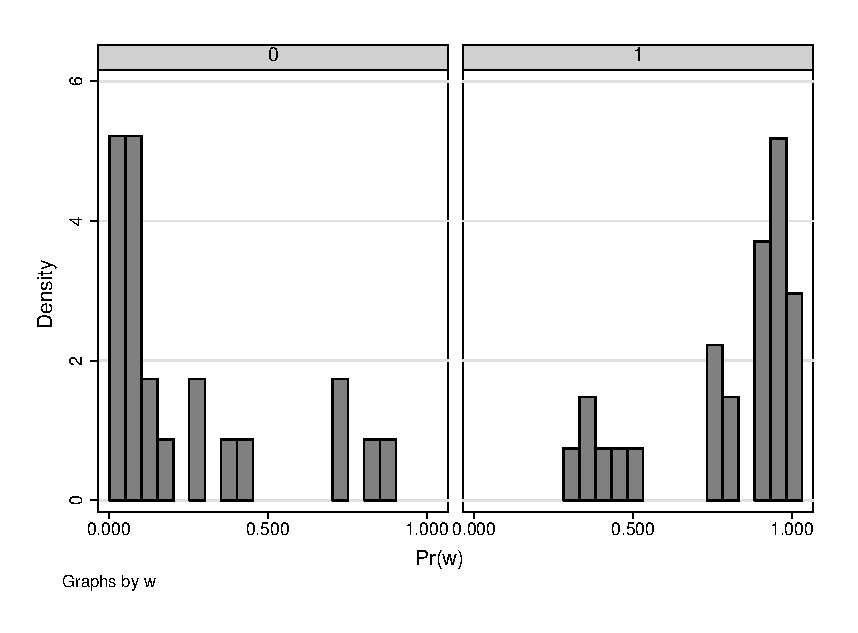
\includegraphics[angle=0,
           width=.75\textwidth]{propplot.eps}
   \caption{Propensity scores from Table~\ref{tab:propensity} by assignment variable $w$ }
  \label{fig:propplot}
\end{figure}

\section*{For more information}
For comprehensive treatment of causal inference and propensity score methods, see \citep{qed} and \citep{rosenbaum1983central}. For discussion of quasi-experimental design and observational studies, consult \citep{kenny1975quasi} and \citep{imbens2004}. Additional perspectives on matching and weighting methods can be found in \citep{freedman2008weighting} and \citep{caliendo2008some}.